\documentclass{article}

\usepackage{times}
\usepackage{uist}
\usepackage{graphicx}

\begin{document}

% --- Copyright notice ---
\conferenceinfo{UIST'08}{October 19--22, 2008, Monterey, CA, USA.}
\CopyrightYear{2008}
\crdata{x-xxxxx-xxx-x/xx/xxxx}

% Uncomment the following line to hide the copyright notice
\toappear{}
% ------------------------

\bibliographystyle{plain}

\title{HoverCross: A New Selection Paradigm for Pen-Based Interfaces}

%%
%% Note on formatting authors at different institutions, as shown below:
%% Change width arg (currently 7cm) to parbox commands as needed to
%% accommodate widest lines, taking care not to overflow the 17.8cm line width.
%% Add or delete parboxes for additional authors at different institutions. 
%% If additional authors won't fit in one row, you can add a "\\"  at the
%% end of a parbox's closing "}" to have the next parbox start a new row.
%% Be sure NOT to put any blank lines between parbox commands!
%%

\author{
\parbox[t]{5cm}{\centering
	     {\em Alice Zhu}\\
	     Harvey Mudd College\\
             Claremont, CA\\
	     xzhu@hmc.edu}
\parbox[t]{5cm}{\centering
	     {\em Scott Parkey}\\
	     Harvey Mudd College\\
	     Claremont, CA\\
	     sparkey@hmc.edu}
\parbox[t]{5cm}{\centering
	     {\em Christine Alvarado}\\
	     Harvey Mudd College\\
	     Claremont, CA\\
	     alvarado@cs.hmc.edu}
}

\maketitle

\abstract A central problem in pen-based interfaces is how to
transition smoothly between drawing and editing.  Separate drawing and
editing modes can be awkward and distracting, while modeless editing
gestures are error-prone.  We present HoverCross, a seamless inking and
editing interface that provides a simple and reliable method for users
to select on-screen objects.  HoverCross
combines the strengths of several recent developments in pen-based
interfaces.  With HoverCross, users ink normally and then select
objects or ink strokes by crossing over them in the hover space above
the tablet screen.  They can then edit their selection through a
context menu on the canvas.  User feedback indicates
that HoverCross provides a promising new pen-based selection technique that offers an efficient, fluid and robust transition
between drawing and editing.

\classification{H5.2 [Information interfaces and presentation]:
User Interfaces. - Graphical user interfaces.}

\terms{Design, Human Factors}

\keywords{Hover space, pen input, tablets.}

\tolerance=400 
  % makes some lines with lots of white space, but 	
  % tends to prevent words from sticking out in the margin

\section{INTRODUCTION}

The promise of pen-based interfaces is that they provide a natural way
for users to create diagrams and take free-form notes.  However, the
integration of diagram creation and diagram editing remains a barrier
to the widespread use of these interfaces.  Pens are more convenient
and natural for drawing, but editing with a pen remains cumbersome
when the user is forced to rely on graphical user interfaces designed
for a mouse and keyboard.  Because the user must use the pen for both
drawing and editing (or suffer the inconvenience of switching between
the pen and the keyboard), a core challenge for pen-based computing is
to construct an interface that allows users to switch easily between
the two tasks, while allowing the system to unambiguously interpret a
given pen stroke as drawing or editing.

Many people have proposed solutions to this problem in recent years.  Traditional solutions (e.g., Windows Journal) require the user to
enter ``edit mode,'' usually by pressing a software button.  This
solution is simple, but the problems with modes are well
known~\cite{Tesler1981Smalltalk}.  Using hardware buttons (e.g., the
bezel buttons on the side of the Tablet PC) to trigger mode switching
helps solve these issues because the mode switch is temporary---as
soon as the user releases the button, the interface reverts to drawing
mode.  Thus, there is little potential for mode confusion.  Studies
suggest that this approach can be quite effective and
natural~\cite{Li2005Experimental,Hinckley2006Springboard}.  However,
simply pressing the button requires not only extra physical effort,
but in many cases also an extra hand.

Other researchers take a recognition-based
approach~\cite{Saund2003Stylus,Zeleznik2006Fluid}, attempting to distinguish
automatically between drawing and editing strokes (e.g., lasso
selections or gestures).  However, even with choice
mediators~\cite{Mankoff2000Providing} to help resolve recognition
ambiguities, recognition errors can be confusing.  Furthermore, as we
argue below, it is not clear that lasso selection is optimal for many
selection tasks.

Recently, researchers have explored using the hover space\footnote{The
\textit{hover space} is the space above the surface of a digital
tablet where the pen is still tracked but does not generate ink or
mouse events.} to invoke editing commands.  Grossman et al. present
Hover Widgets~\cite{Grossman2006Hover}, in which the user performs
gestures in the hover space to activate editing menus.  Following on
this work, Subramanian et al. explore the possibility of using several
layers of the hover space to perform different editing
tasks~\cite{Subramanian2006Multilayer}, while Kattinakere et
al. formally model users' ability to track (e.g., execute gestures) in
hover space \cite{Kattinakere2007Modeling}.


While each of these recently developed approaches brings us closer to
the dream of seamless pen-based drawing and editing, we believe our
arsenal of drawing and editing techniques is not yet complete.  Specifically, for common diagram creation and editing tasks, Hover
Widgets or a multi-level hover space solution may be too heavyweight.

We explore the power and simplicity that can be obtained by combining
the simplest aspects of many existing techniques.  Our interface,
called HoverCross, combines the strengths of hover space editing and
crossing-based selection (e.g.,~\cite{Apitz2004Crossy}),
resulting in an interface that is easy to learn, reliable, and fast
for common drawing and editing tasks.  Furthermore, our
approach integrates seamlessly with almost any other pen-based editing
technique, so in the worst case users can simply ignore it and fall
back on traditional editing methods.

%% Advantages of our approach: Simple, easy to learn, relatively little
%% chance of recognition error, integrates seamlessly with other
%% techniques, powerful (preferred by some users and faster than other
%% techniques for some common tasks).

%% Our interface provides
%% only one simple, reliably recognized gesture for the user to remember,
%% and this gesture is performed on the canvas so the user does not need
%% to learn to make it in hover space.  \textit{This paragraph is key and
%% needs some work.  The main contributions are that the hover space is
%% not overloaded so you don't need to use gestures in it.  Selection is
%% the number one thing you want to do in editing, and in effect it is a
%% precursor to all other editing things, so you just have to provide
%% support for that, and then you can leverage the fact that when
%% something is selected the user is probably editing.}  

%% I took this text out, but I want it around because it's nicely
%% phrased and I may have lost some of it when I wrote the text above.

%% We propose a new interface not only for creating and manipulating
%% objects with a stylus, but also for transitioning seamlessly between
%% the two tasks. Our work builds on and combines several existing
%% ideas. First, Grossman et al. explore the hover space  for diagram
%% editing [2]. We propose using this space to trigger selection reliably
%% and conveniently. To perform selection in the hover space, we use a
%% crossing metaphor, explored in CrossY, [3] as a substitute for the
%% traditional point-and-click interaction. To manipulate the selection,
%% we use a simple gesture performed on the Tablet screen to bring up a
%% ring-shaped menu around the location of the pen, as described in
%% Scriboli [4].


\section{INTERACTION USING HOVERCROSS}

In many modal pen-based interfaces (e.g., Windows Journal), it is
\textit{selection}, not editing in general, that typically
operates in its own mode.  This division makes sense, as selecting
objects in a drawing is typically the first step in performing almost
any editing task.  Once the user selects an object, she can edit it
via a menu or direct manipulation.  An explicit selection mode seems
necessary because any apparent selection stroke just as easily could
be a drawing stroke.

The key insight behind HoverCross is that relegating the process of
selection to the hover space allows users to switch seamlessly between
drawing and selecting without pressing any buttons.  Furthermore,
because the user performs only selection in the hover space, a simple
crossing interface suffices, and there is no need to perform gestures
in the hover space.  The system then leverages the context of the
selection to give the user additional power through a
gesture-invoked context menu or direct interaction with the selected
objects.

In our interface, the user draws normally on the screen to create
diagrams containing simple shapes, text, and ink.  The Microsoft gesture and text
recognition engines recognize the diagrams and text the
user draws, while the unrecognized ink becomes one selectable object per stroke.

To edit the diagram, the user hovers the pen briefly over the tablet
to trigger selection.  The brief pause prevents triggering selection
every time the stylus enters the range, as it inevitably does on its
way to the screen.  The length of the pause therefore affects whether users accidentally enter into selection or must wait too long; half a second appears to work as a medium.  Once the user triggers selection, a small vertical line, called the handle,
appears in the middle of each object, anchored at the bottom (Figure~\ref{fig:handles}).  The vertical alignment keeps the selection gesture a horizontal motion, which is intuitive because it is similar to horizontal motion while writing.

The user simply needs to cross the stylus over the handle in either
direction in hover space to select the object.  Once the object is selected, the handle 
realigns its anchor to the top of the shape, creating a switch-like
feel, which helps prevent users from accidentally undoing their selection and keeps
handles from becoming too obstructive (Figure~\ref{fig:selection}).  Crossing the realigned handle
deselects the shape.  The user can easily cross over multiple objects to select all
of them.  To clear the selection, the user moves the pen in hover
space off the edge of the screen.

HoverCross also draws small circles and squares on the edge of shapes when the user enters selection mode.  Clicking and dragging these small shapes causes the shapes to transform: the square will resize the corresponding object, and the circle will rotate the corresponding object.  These mimic existing transformation techniques used by programs such as PowerPoint and Visio.  So, they are not a new development, nor are they unique to HoverCross.  However, their presence demonstrates that common transformation tools do not conflict with the new selection interface.  Since selection occurs in the hover space, while transformation occurs when the pen is down, attempting to select objects will not accidentally transform them, nor will attempting to transform objects accidentally select them.

The user can enter the hover
space to cross one object and then immediately exit the hover space by
moving the pen tip away from the screen.  The selected object remains
selected even when the pen is outside of hover space.  To select
another object, the user simply needs to re-enter hover space near
that object.  This ability helps keep intervening handles between two
desired objects from preventing the user from selecting both.

\begin{figure}[tb]
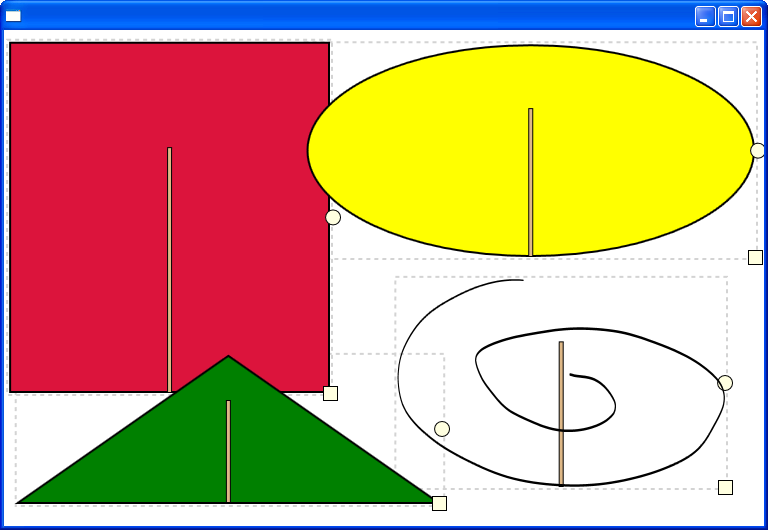
\includegraphics[width=3.0in]{SelectionHandlesOn}
\caption{Vertical bars appear on each object to give users a crossing
  target.} 
\label{fig:handles}
\end{figure}

\begin{figure}[tb]
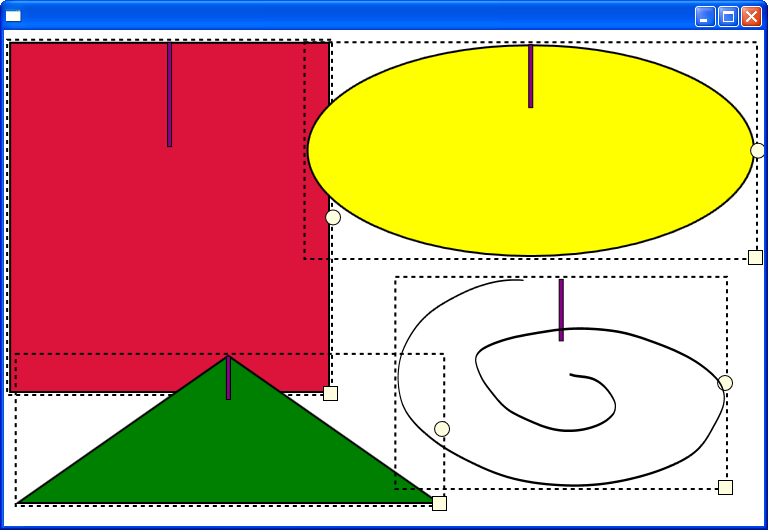
\includegraphics[width=3.0in]{SelectedObjects}
\caption{How selected objects appear.}
\label{fig:selection}
\end{figure}


Once the user has selected at least one item, she can either edit the
selected item, or continue to draw new portions of the diagram.  The
user has several options for editing the diagram.  She can move
selected shapes by dragging one of them with her pen on the
screen.  As long as she does not cross the handle in hover space,
touching the shape will not deselect it.  For more complicated
editing tasks, the user can bring up a context menu
around the tip of the stylus (Figure~\ref{fig:contextMenu}).  The implementation of the menu is tangential, since any menu could work.  We have altered the gesture for bringing up the menu; currently, it requires the user to hold the stylus down, utilizing the straightforward and well-known Windows right-clicking gesture.  The
content of the menu depends on the type of objects selected, such
as text or shapes.  The user can navigate the menus by tapping the stylus on the menu options to quickly manipulate the selection.  With little
practice, the user can easily coordinate drawing, selecting, and
editing in one fluid motion.

\begin{figure}[tb]
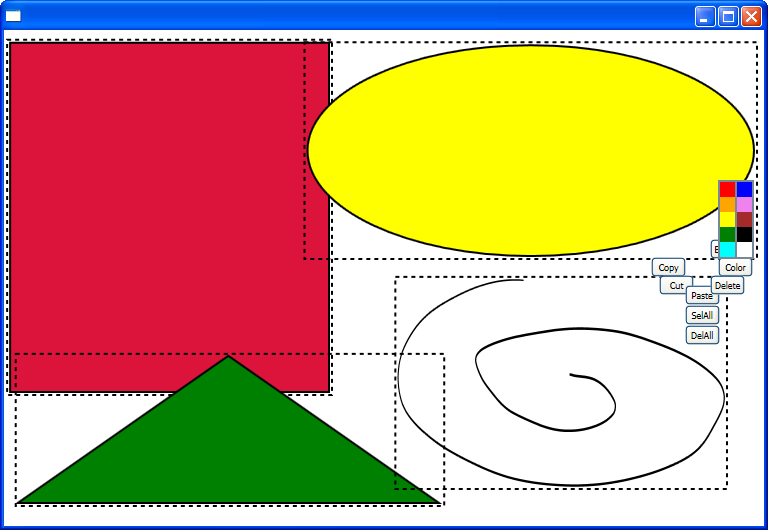
\includegraphics[width=3.0in]{ColorMenu}
\caption{The context menu that appears when the user makes a simple
  gesture.  The menu appears at the tip of the stylus at the end of
  the gesture, and actions apply to all selected shapes and strokes.}
\label{fig:contextMenu}
\end{figure}

\section{DESIGN DECISIONS}
The design of HoverCross focused on giving users the ability to seamlessly transition between drawing and editing mode within a diagram-editing paradigm. We also conducted several preliminary user tests to determine the effectiveness of HoverCross, and adjusted our design based on their results.  We confirmed several strengths about HoverCross upon implementation and after performing the users tests, including its extensibility and its ability to easily work with objects lying in a row.  However, we also discovered problems associated with very tall and short objects, and with objects grouped on top of each other, and took steps to mediate these problems.

\subsection{Preliminary User Tests}

In the first user test, we compared three selection interfaces: an older version of HoverCross that utilized much of the existing functionality, including crossing selection; a variation of
HoverCross called Cross; and the traditional lasso select.  Cross
differs from HoverCross in that users cross objects with the pen on
the screen while holding down a nonpreferred hand button.  Li et
al. showed that using a nonpreferred hand button is the current most
effective way to invoke edit mode~\cite{Li2005Experimental}.  Lasso
select invoked using a modal interface button is the current approach
in most commercial software.  Seven users (3 female and 4 male) participated in this study.  All were students at Harvey Mudd College, and all had experience using
a tablet computer.  No user had experience with a hover or
crossing-based interface.  After receiving instructions and trying out the three interface
techniques for about 2-5 minutes, users performed four tasks using
each of the three interface techniques.

In the latter tests, we told users to simply draw a picture, some of which became fairly complex and included shapes overlapping other shapes.  These pictures approximate the complexity of a typical diagram or PowerPoint slide, which will often include several overlapping shapes.

\subsection{Strengths}

The HoverCross technique is appropriate for any application that
combines pen-based drawing and editing.  Our example application
supports the creation of clean diagrams that combine shapes and text,
such as might be produced in PowerPoint or Visio.  We chose this
domain because creating polished diagrams typically requires more
intensive editing than simply drawing freeform notes and diagrams.  In
a previous pilot study in which we observed people creating slides in
PowerPoint, we found that they relied heavily on copying, pasting,
resizing and moving shapes within their diagrams.  This domain thus
allows us to evaluate the utility of HoverCross for its intended
purpose.

Confirming previous results~\cite{Apitz2004Crossy}, the crossing
selection metaphor has several advantages over traditional lasso
selection.  For selecting single shapes or shapes roughly in a
horizontal row, preliminary user tests have suggested that crossing the shapes' handles is much faster than
lassoing the shapes.  Additionally, for shapes spread out in space, crossing
in hover space behaves like ``Control-clicking'' with a mouse and
keyboard, allowing users to select some objects while avoiding
intervening ones.

A final strength of this interface is that any part of it may be
implemented in conjunction with almost any other interface technique.  If the user does not want to use it, he can simply ignore it.  Because
the hover selection interface requires a short pause to invoke, the
user is not likely to trigger it by mistake, so it may be combined
with a traditional modal selection interface.  For example, a user
might use modal lasso selection to select a group of tightly clumped
objects, and then use HoverCross to deselect one of them.  While we
offer the context menu for convenience, additional menus may be added
easily to the interface.

\subsection{Differently Shaped Objects Problem}

A common problem we discovered in the first user tests was that if handles are the same height as their shapes, they would either be too easily selected or too difficult to select if the shapes were either too tall or too short.  So, rather than having the selection handles fit the shapes precisely, we gave the handles minimum and maximum sizes.  We also made the handles switches that change position and color depending on whether their shape is selected to facilitate user interaction, so the handles could never extend across the entire shape.  Users in latter tests approved of the switch paradigm, and frequently commented that although it took some time to get used to, object selection became natural and fit well with the drawing system.

\subsection{Occluded Shapes Problem}

Another common problem we found in early user tests was the fact that shapes obstructed by other shapes would be either difficult or impossible to select.  We fixed this problem by counting crosses over obstructed handles as legitimate crosses.  This improvement consistently tested well when given to users for feedback.  Although allowing crossing selection of obstructed shapes was worrisome for the accidental selections it may produce, users rarely cited it as a problem, in contrast with the negative feedback we received about the inability to select obstructed shapes.

Still, this improvement gave rise to another complication in the user tests, when shapes were grouped directly on top of other shapes.  For example, if one handle became grouped directly on top of another handle, the user would switch them both simultaneously when they cross them.  Although annoying, this was never a critical flaw, because users could simply resort to another means of selection, such as tapping the rotation circle and moving the shape on top.  It is also worth noting that lasso selection does not solve this problem, either, since lassoing would always select both shapes as well.  Indeed, HoverCross is probably an improvement in precision over lasso selection for cluttered diagrams, since the selection process is precise to a single, visible line segment.

\section{USER FEEDBACK AND FUTURE IMPROVEMENTS}

Our preliminary user tests consistently reflected that users enjoyed the
transition between sketching and selecting, without the hassle of
pressing a button or other explicit indication, despite the
reliability of the button.  In addition, for small selections, users said that drawing
a circle around the objects seemed excessive.  When objects were spread
out over the canvas, they felt that selecting a few of them with lasso
select was awkward, while with HoverCross they could simply move the
pen across the screen to the objects of interest.  This result suggests that
there is a set of users that would benefit greatly from HoverCross in
this situation.

Our first preliminary user test involved four tasks.  We collected qualitative data on which interface users preferred for each task.  For these same tasks, four users preferred HoverCross over the other
two interfaces (Figure~\ref{tab:pref}).  Only in task 2, which involved selecting a group of closely placed objects, did users tend to prefer lasso select to crossing.  This result is
understandable, because crossing over each individual object in the
group is more cumbersome than drawing a lasso around it.  However, one
user still preferred HoverCross for this task.  He reflected that,
while both interfaces are effective, HoverCross was more interesting
and fun.

\begin{figure}
\begin{center}
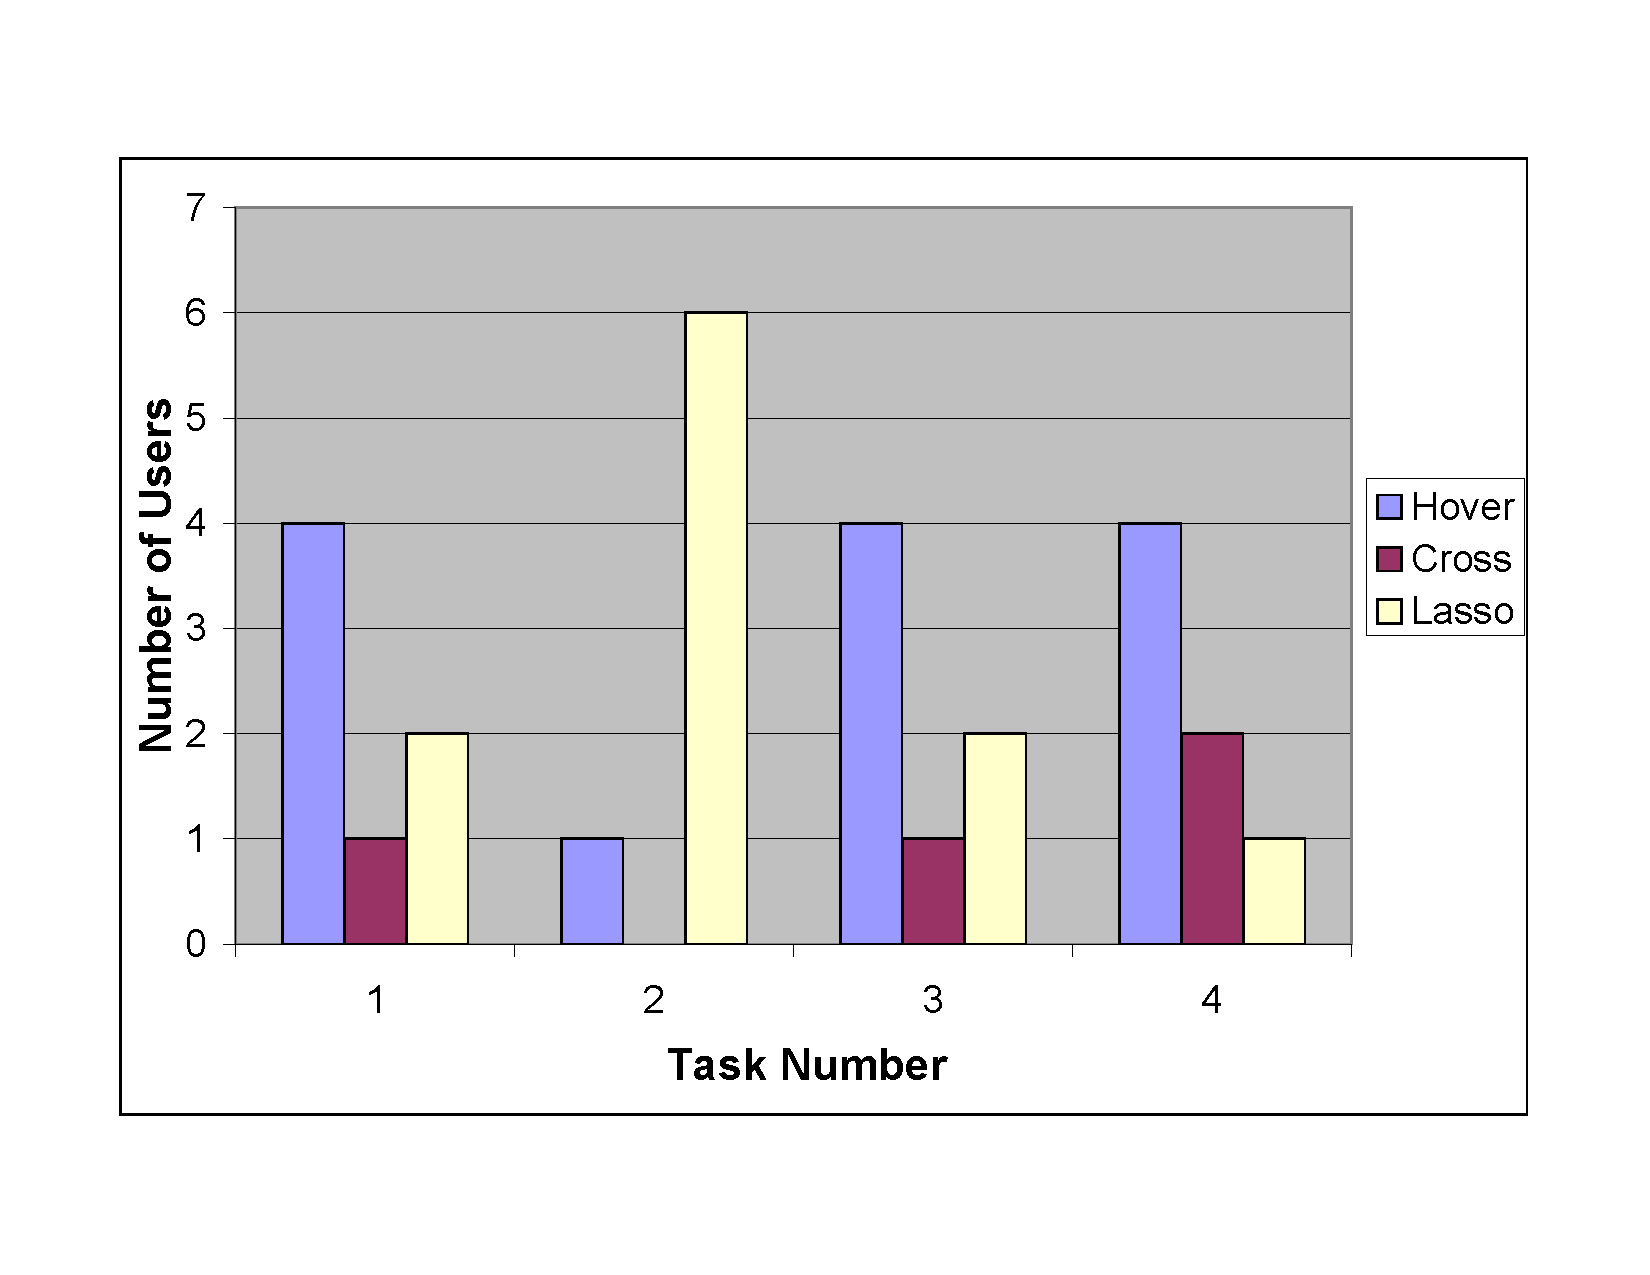
\includegraphics[width=3.0in]{Preferences}
\caption{Number of users who preferred each interface for each task.}
\label{tab:pref}
\end{center}
\end{figure}

The need for improvements to HoverCross remains.  Users occasionally complained about the selection boxes becoming too cluttered, particularly for diagrams with many small strokes; we could address this problem by grouping strokes.  Although the selection mode is effectively in its final stages of implementation, the rest of the prototype could use improvements in text recognition, menu access, and graphical issues.  In addition, before we can make any positive claims about the effectiveness of the selection mode when deployed into other environments, we must deploy it into other environments and conduct more formal user studies.

\section{IMPLEMENTATION}

This interface, designed for the Tablet PC, is written in C\# using
Windows Presentation Foundation and .NET 3.0.  We use the built-in
gesture and text recognizers.  We recognize movement in the hover
space by handling the StylusInAirMove event, tracking the stylus
position, and selecting or deselecting an object whenever the stylus
crosses its handle.

HoverCross determines whether or not a motion crosses a handle by storing the previous stylus location and passing it, along with the current stylus location, to an intersection test.  The intersection test checks whether the line segment between the two points crosses the center of any handles.  If it does, the method returns all the handles that the motion crosses.

Our context menu is a
collection of Button UIElements stored on the InkCanvas, each
representing an editing option.  When the user clicks on any of the
buttons, the system performs the desired option on all selected items.

\section{CONCLUSION}
HoverCross combines many simple and effective ideas from many
recent advances in pen-based interfaces to provide an elegant
interface for inking and editing.  Used in combination with other
pen-based interaction techniques, HoverCross will bring us one step
closer to the goal of creating pen-based interfaces that combine the
freedom of paper with the power of the computer in a useful, and
usable, way.  

% use \newpage to break the columns on the last page so they have equal length
% if the break occurs in the middle of a paragraph, insert \linebreak before \newpage
%\linebreak
%\newpage

\section{ACKNOWLEDGEMENTS}
We would like to thank our users who helped us evaluate HoverCross.  Much of this work was funded by the Baker Foundation and an NSF CAREER award
(IIS-0546809).

%%%	You can use bibtex if you like, but I've hardwired in these 
%%%	references to avoid sending you a separate .bib file.
\bibliography{uist08}



\end{document}
